%versi 2 (8-10-2016)
\chapter{Landasan Teori}
\label{chap:teori}
Pada bab ini dijelaskan dasar-dasar teori mengenai \textit{Wireless Sensor Network}, transfer data pada wireless sensor network, prinsip \textit{reliable data transfer} pada Wireless Sensor Network, dan pengembaganan pemrograman pada WSN.

\section{Wireless Sensor Network}
\label{sec:wsn}
\textit{Wireless Sensor Network} merupakan jaringan nirkabel yang terdiri dari sekumpulan \textit{sensor node} yang diletakan pada suatu tempat dan memiliki kemampuan untuk mengukur kondisi lingkungan sekitar(\textit{sensing}), komputasi dan dilengkapi dengan alat komunikasi \textit{wireless} untuk komunikasi antar \textit{sensor node}. Sensor ini akan mengumpulkan data dari kondisi lingkungannya, seperti: cahaya, suara, kelembapan, getaran, gerakan, temperatur, tekanan udara, kualitas air, komposisi tanah, dan lain-lain. Data ini kemudian dikirimkan ke \textit{sensor node} tetangganya hingga sampai ke \textit{base station} sebagai pusat untuk dikelola.

\subsection{Penerapan Wireless Sensor Network}
Pada awalnya \textit{sensor network} (jaringan sensor) digunakan dalam teknologi militer untuk mendeteksi musuh di laut dan di darat. Semakin lama sensor node ini banyak dikembangkan untuk membantu berbagai bidang kehidupan manusia. Pemanfaatan Wireless Sensor Network pada kehidupan manusia dapat dilihat pada ilustrasi Gambar~\ref{fig:smartworld}. Berikut adalah beberapa penerapan wireless sensor network pada berbagai bidang kehidupan manusia:
\begin{itemize}
\item Bidang militer\\
Wireless Sensor Network digunakan sebagai bagian dari komunikasi pada bidang militer dan deteksi target atau musuh.

\item Monitoring area\\
Pada monitoring area, sensor node akan disebar pada suatu tempat yang akan di monitoring. Saat sensor node mendeteksi suatu kejadian(panas, tekanan, dan lain-lain) pada tempat, data akan dikirimkan ke base station untuk ditentukan tindakan selanjutnya.

\item Transportasi\\
Pada bidang transportasi wireless sensor network digunakan untuk mendeteksi lalu lintas secara aktual yang nantikan akan disampaikan kepada pengendara tentang kejadian di depan mereka seperti kemacetan lalu lintas. 

\item Kesehatan\\
Beberapa aplikasi kesehatan seperti membantu pada disabilitas, monitoring pasien, diagnosis, pengaturan penggunaan obat, dan pelacakan dokter dan pasien di rumah sakit.

\item Deteksi lingkungan\\
Deteksi lingkungan yang dapat dilakuan antara lain deteksi gunung berapi, polusi udara, kebakaran hutan, efek rumah kaca, dan deteksi longsor.

\item Monitoring struktur\\
Wireless Sensor Network dapat melakukan deteksi pergerakan bangunan dan infrastruktur seperti jembatan, flyover, terowongan dan fasilitas lain tanpa mengeluarkan biaya untuk melakukan dektesi manual dengan mendatangi tempatnya secara langsung.

\item Bidang pertanian\\
Pada bidang pertanian dapat membantu pengelola pertanian untuk mengelola penggunaan air dalam irigasi dan menghasilkan lebih sedikit hasil buangan dari pertanian mereka.
\end{itemize}

\begin{figure} [H]
	\centering  
	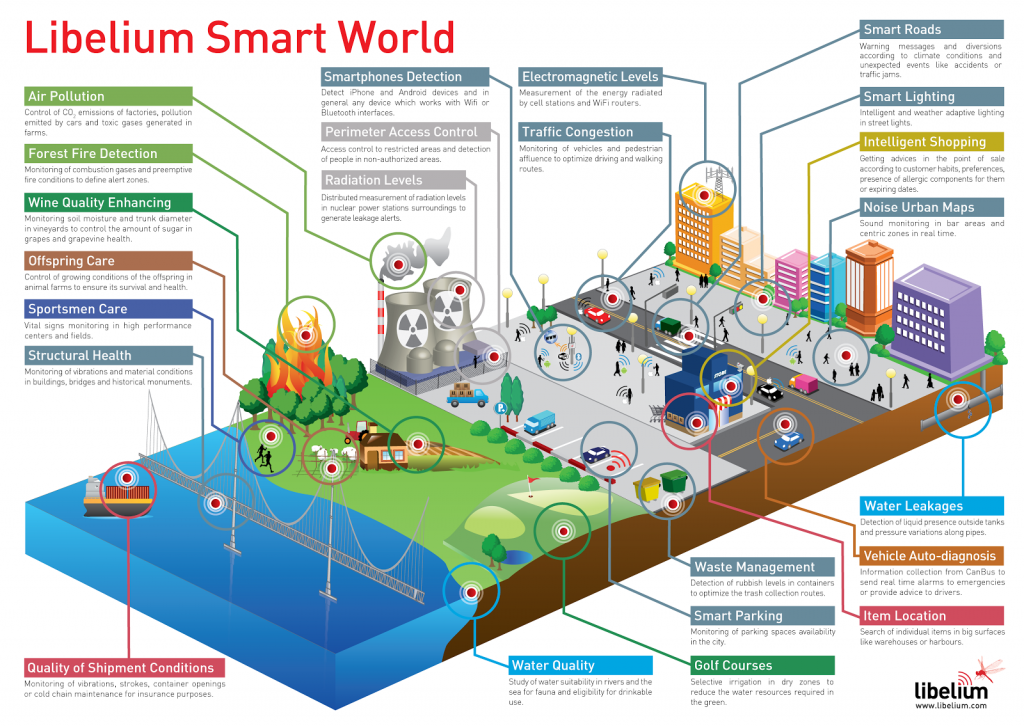
\includegraphics[scale=0.4]{libelium_smart_world}  
	\caption[Pemanfaatan \textit{Wireless Sensor Network} diberbagai bidang kehidupan manusia]{Pemanfaatan \textit{Wireless Sensor Network} diberbagai bidang kehidupan manusia} 
	\label{fig:smartworld} 
\end{figure} 

\subsection{Struktur Wireless Sensor Network}

\subsection{Arsitektur Wireless Sensor Network}
Pada \textit{Wireless Sensor Network} biasanya akan terdapat banyak \textit{sensor node} yang disebar pada suatu tempat atau daerah, dan terdapat satu atau lebih \textit{sink node} atau \textit{base station} dalam area sensing tersebut (Gambar~\ref{fig:libelium_smart_world}). Dalam membuat \textit{Wireless Sensor Network} perlu diperhatikan arsitektur yang akan digunakan. Arsitektur jaringan yang biasanya dipakai pada \textit{Wireless Sensor Network} adalah \textbf{arsitektur flat} dan \textbf{arsitektur hierarki}. Selain itu dalam membangun \textit{Wireless Sensor Network} perlu juga diperhatikan jalur lintasan yang menghubungkan antar \textit{sensor node} saat transfer data. Untuk area \textit{sensing} yang tidak terlalu luas dan hanya menggunakan sedikit \textit{sensor node} dapat menggunakan protokol routing \textbf{\textit{single hop}}. Sedangkan untuk daerah yang luas dan memerlukan banyak \textit{sensor node} dapat menggunakan protokol routing \textbf{\textit{multi hop}}. 

\subsubsection{Single-Hop dan Multi-Hop}
Untuk mengirim data ke sink node setiap sensor node dapat menggunakan single-hop long-distance transmission. Single-hop long-distance ini berarti setiap sensor node akan mengirimkan data ke sink node hanya satu kali lompatan walaupun jarak antara sink node dengan sensor node itu sangat jauh. Dalam jaringan sensor, pengguanaan daya paling besar adalah saat melakukan komunikasi dibandingan saat sensing. Penggunaan daya akan semakin bertambah jika jarak sink dan sensor node semakin jauh. Untuk menangani masalah tersebut muncul protokol multi-hop.

Pada protokol multi-hop sensor node akan disusun saling berdekatan dan terhubung dengan yang lain. Jadi saat akan berkomunikasi dengan sink node, sensor node harus mengirimkan data tersebut ke sensor node tetangganya dan diteruskan hingga sampai ke sink node. Karena jarak yang saling berdekatan maka penggunaan daya dapat efektif. Single-hop dan multi-hop ini dapat digunakan dengan arsitektur flat maupun hierarki sesuai dengan kebutuhan sistem.


\subsubsection{Arsitektur Flat}
Pada jaringan flat, setiap \textit{sensor node} memiliki peran / \textit{role} yang sama dalam melakukan \textit{sensing}. Secara fungsional hanya terdapat dua macam \textit{sensor node} pada jaringan flat, yaitu \textit{source node} dan \textit{sink node}. Karena jumlah \textit{sensor node} yang banyak maka tidak mungkin menentukan \textit{global identified} untuk setiap \textit{sensor node} pada jaringan ini. Untuk mendapatkan data dilakukan dengan cara \textit{sink node} melakukan transmit ke semua \textit{sensor node} pada area \textit{sensing} dengan cara \textit{flooding} dan hanya \textit{sensor node} yang sesuai yang akan merespon \textit{sink node}. Setiap \textit{sensor node} mengirimkan data ke \textit{sink node} dengan \textit{multi hop} dan melalui node tetangganya yang terhubung dengannya untuk meneruskan data (Gambar~\ref{fig:libelium_smart_world}). Arsitektur flat juga dapat dilakukan dengan \textit{single hop} seperti pada Gambar~\ref{fig:libelium_smart_world}.
% gambar flat multihop
\begin{figure} [H]
	\centering  
	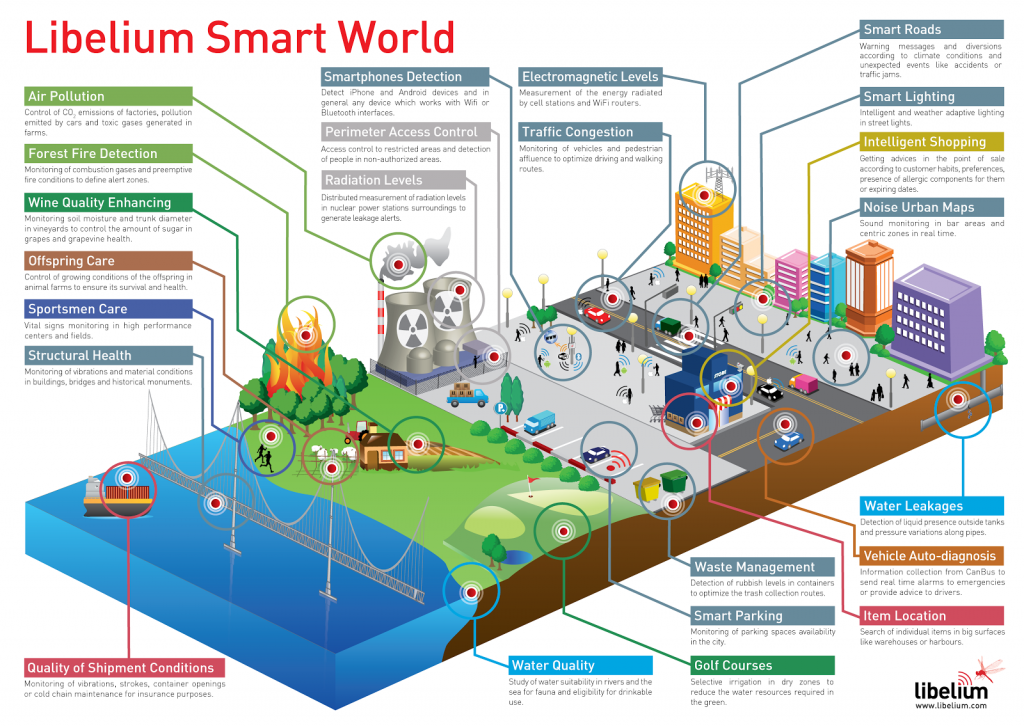
\includegraphics[scale=0.2]{libelium_smart_world}  
	\caption[Ilustrasi arsitektur flat pada \textit{Wireless Sensor Network} dengan \textit{multi hop}]{Ilustrasi arsitektur flat pada \textit{Wireless Sensor Network} dengan \textit{multi hop}} 
	\label{fig:libelium_smart_world} 
\end{figure} 
% gambar flat singlehop
\begin{figure} [H]
	\centering  
	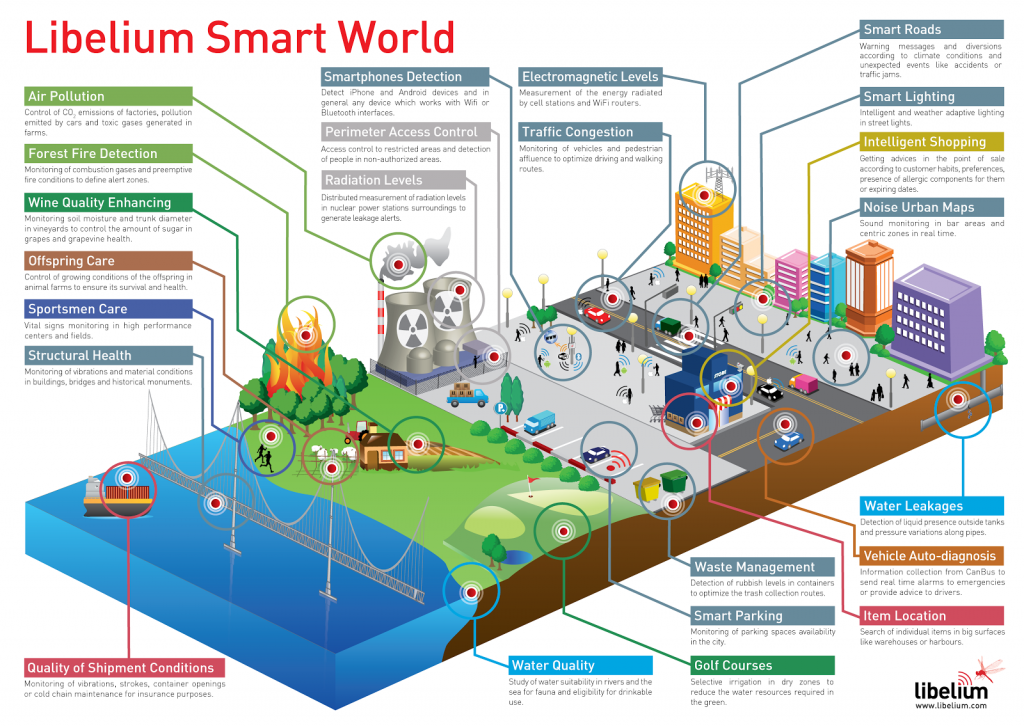
\includegraphics[scale=0.2]{libelium_smart_world}  
	\caption[Ilustrasi arsitektur flat pada \textit{Wireless Sensor Network} dengan \textit{single hop}]{Ilustrasi arsitektur flat pada \textit{Wireless Sensor Network} dengan \textit{single hop}} 
	\label{fig:libelium_smart_world} 
\end{figure} 

\subsubsection{Arsitektur Hierarki}
Pada arsitektur hierarki, semua sensor node dikelompokan ke dalam cluster-cluster. Terdapat cluster head pada setiap cluster. Cluster head ini yang mengumpulkan data dari setiap sensor node di bawahnya dan meneruskan data yang telah diterima ke base station atau sink. Hal yang perlu diperhatikan pada arsitektur hierarki adalah pemilihan sensor node sebagai cluster head dan sensor node yang melakukan sensing. Penggunaan daya yang paling besar dalam Wireless Sensor Network ini adalah saat melakukan komunikasi yaitu saat mengirimkan data ke sensor node lain. Maka untuk sensor node yang memiliki daya kecil dapat digunakan untuk sensing, karena sensor node sensing ini hanya melakukan komunikasi ke cluster head. Cluster head harus memiliki daya yang lebih banyak, karena cluster head akan bertugas menerima hasil sensing sensor node di bawahnya dan meneruskan data ke sink node. 

Masalah yang utama pada clustering ini adalah pemilihan cluster head dan bagaimana cara mengatur setiap cluster. Terdapat beberapa cara untuk membuat clustering ini. Bedasarkan jarak antara cluster head dengan cluster member, dapat dibuat clustering dengan single hop atau multi hop seperti pada Gambar~\ref{fig:libelium_smart_world} dan Gambar~\ref{fig:libelium_smart_world}. Sedangkan jika berdasarkan jumlah tier dapat dibangun clustering single tier atau multi tier seperti pada Gambar~\ref{fig:libelium_smart_world} dan Gambar~\ref{fig:libelium_smart_world}.

% gambar cluster multihop
\begin{figure} 
	\centering  
	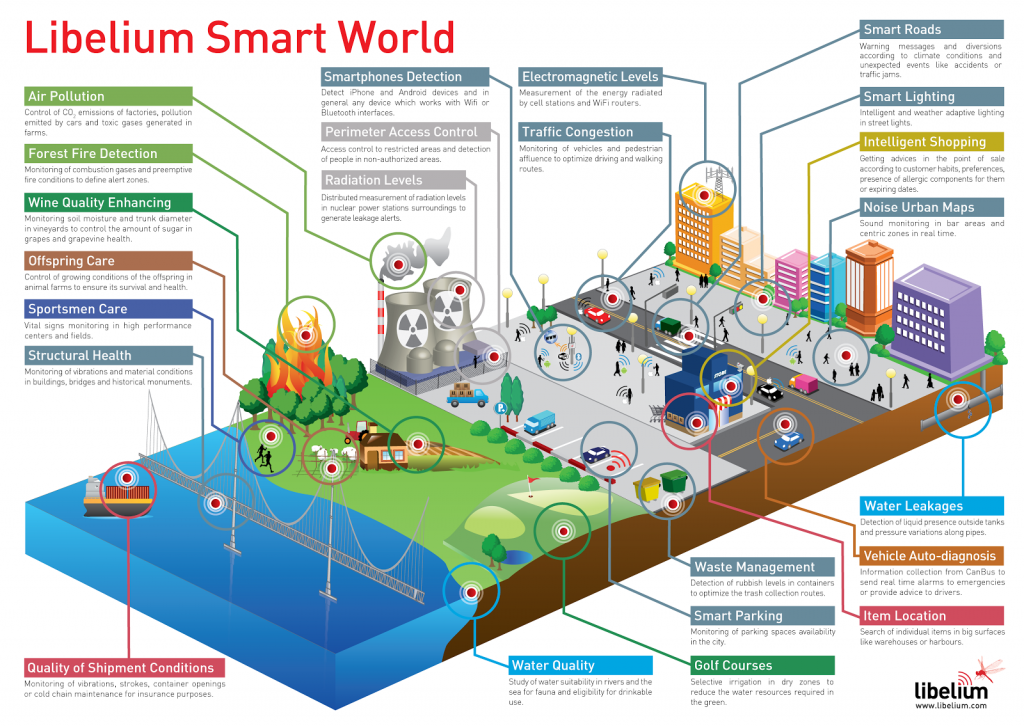
\includegraphics[scale=0.1]{libelium_smart_world}  
	\caption[Ilustrasi arsitektur flat pada \textit{Wireless Sensor Network} dengan \textit{multi hop}]{Ilustrasi arsitektur flat pada \textit{Wireless Sensor Network} dengan \textit{multi hop}} 
	\label{fig:libelium_smart_world} 
\end{figure} 
% gambar cluster singlehop
\begin{figure} 
	\centering  
	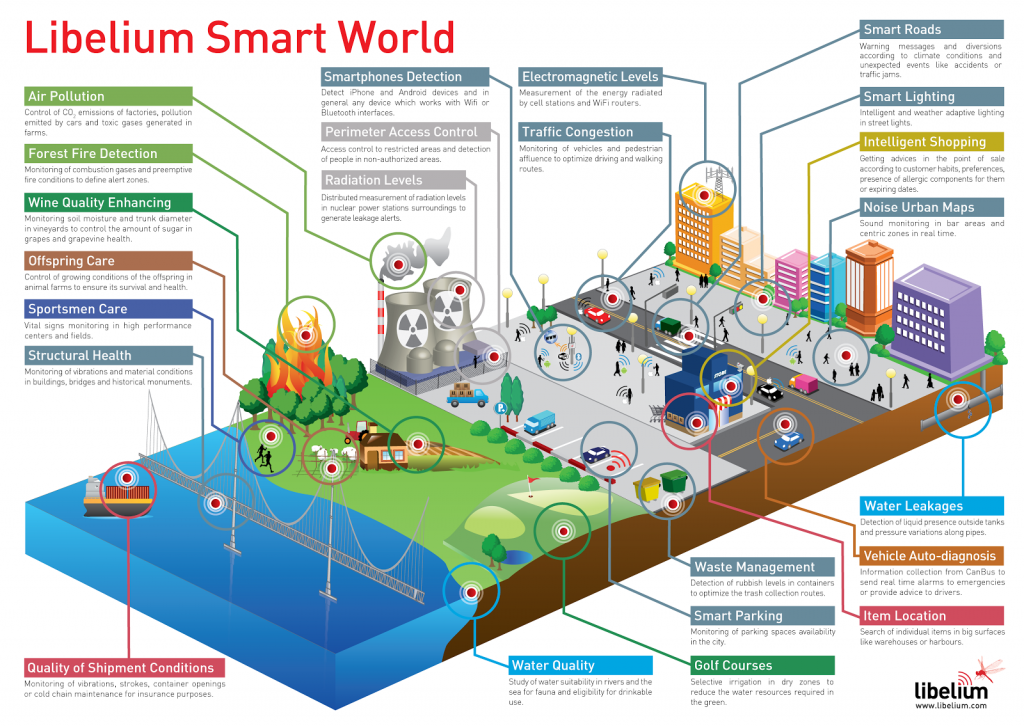
\includegraphics[scale=0.1]{libelium_smart_world}  
	\caption[Ilustrasi arsitektur flat pada \textit{Wireless Sensor Network} dengan \textit{single hop}]{Ilustrasi arsitektur flat pada \textit{Wireless Sensor Network} dengan \textit{single hop}} 
	\label{fig:libelium_smart_world} 
\end{figure} 

% gambar clustering single tier
\begin{figure} [H]
	\centering  
	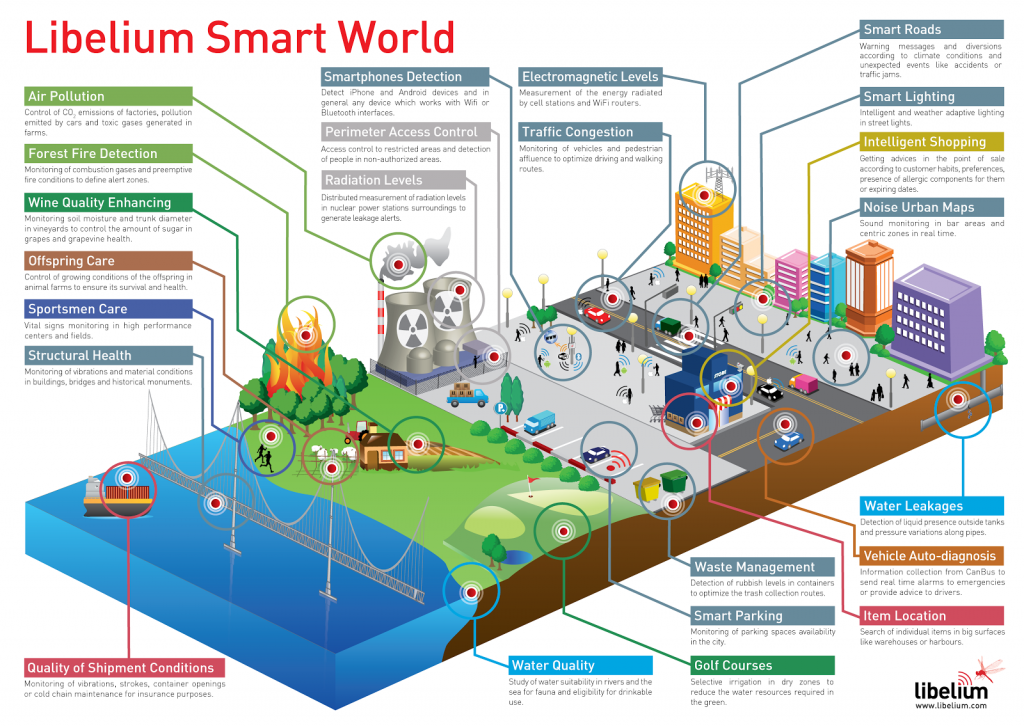
\includegraphics[scale=0.1]{libelium_smart_world}  
	\caption[Ilustrasi clsutering dengan single tier]{Ilustrasi clsutering dengan single tier} 
	\label{fig:libelium_smart_world} 
\end{figure} 
% gambar clustering multi tier
\begin{figure} [H]
	\centering  
	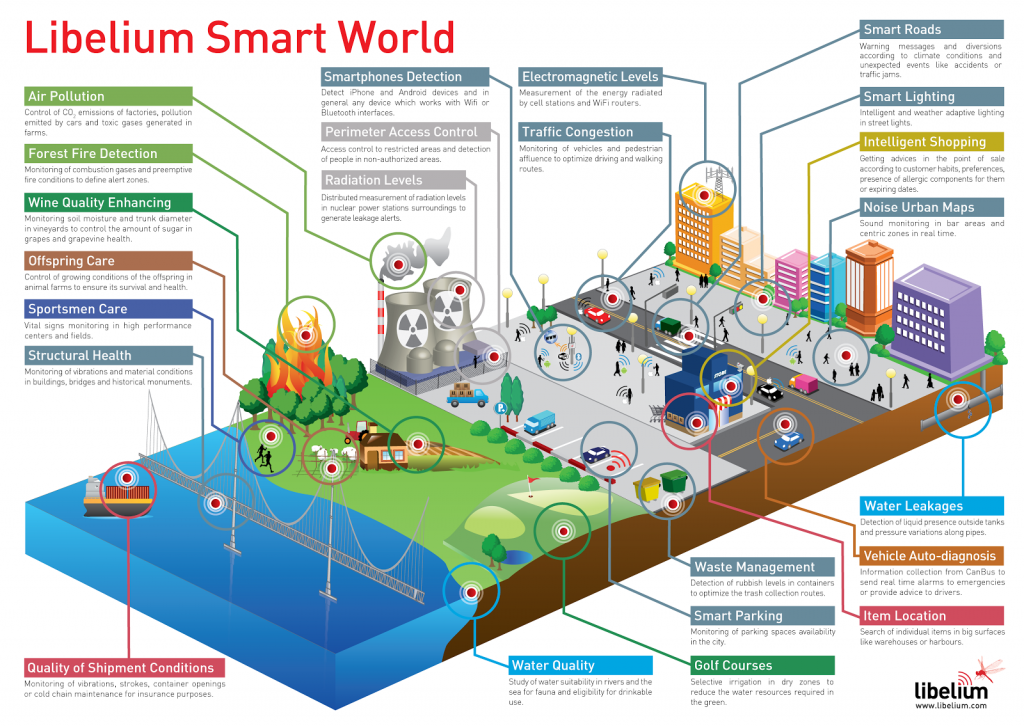
\includegraphics[scale=0.1]{libelium_smart_world}  
	\caption[Ilustrasi clsutering dengan multi tier]{Ilustrasi clsutering dengan multi tier} 
	\label{fig:libelium_smart_world} 
\end{figure}

\subsection{Layer pada Wireless Sensor Network}
Wireless Sensor Network memiliki lima layer protokol: physical layer, data link layer, network layer, transport layer, dan application layer, seperti pada Gambar~\ref{fig:libelium_smart_world}. 


\begin{figure} 
	\centering  
	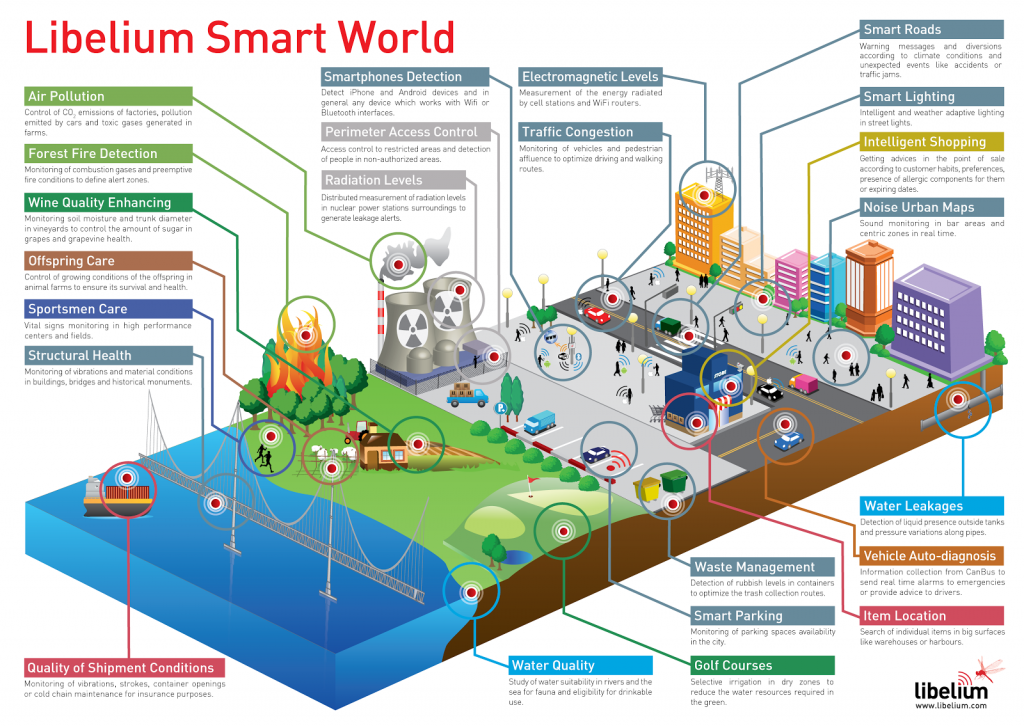
\includegraphics[scale=0.1]{libelium_smart_world}  
	\caption[Layer pada \textit{Wireless Sensor Network}]{Layer pada \textit{Wireless Sensor Network}} 
	\label{fig:libelium_smart_world} 
\end{figure} 

\section{Data Transfer pada Wireless Sensor Network} 
asdf
 
\section{Prinsip Reliable Data Transfer pada Wireless Sensor Network}
\label{sec:reliable}

 
\section{Pengembangan Pemrograman pada Wireless Sensor Network}
\label{sec:pemrograman_wsn}


\newpage
\subsection{Tabel}  
Berikut adalah contoh pembuatan tabel. 
Penempatan tabel dan gambar secara umum diatur secara otomatis oleh \LaTeX{}, perhatikan contoh di file bab2.tex untuk melihat bagaimana cara memaksa tabel ditempatkan sesuai keinginan kita.

Perhatikan bawa berbeda dengan penempatan judul gambar gambar, keterangan tabel harus diletakkan di atas tabel!!
Lihat Tabel~\ref{tab:contoh1} berikut ini:

\begin{table}[H] %atau h saja untuk "kira kira di sini"
	\centering 
	\caption{Tabel contoh}
	\label{tab:contoh1}
	\begin{tabular}{cccc}
		\toprule
		& $v_{start}$ & $\mathcal{S}_{1}$ & $v_{end}$\\

		\midrule
		$\tau_{1}$ & 1 & 12& 20\\
		$\tau_{2}$ & 1 &  & 20\\
		$\tau_{3}$ & 1 & 9 & 20\\
		$\tau_{4}$ & 1 &  & 20\\

		\bottomrule
		
	\end{tabular} 
\end{table}
Tabel~\ref{tab:cthwarna1} dan Tabel~\ref{tab:cthwarna2} berikut ini adalah tabel dengan sel yang berwarna dan ada dua tabel yang bersebelahan. 
\begin{table}[H]
	\begin{minipage}[c]{0.49\linewidth}
		\centering
		\caption{Tabel bewarna(1)}
		\label{tab:cthwarna1}
		\begin{tabular}{ccccc}
			\toprule
			 & $v_{start}$ & $\mathcal{S}_{2}$ & $\mathcal{S}_{1}$ & $v_{end}$\\
			
			\midrule
			$\tau_{1}$ & 1 & 5 \cellcolor{green}& 12& 20\\
			$\tau_{2}$ & 1 & 8 \cellcolor{green}& & 20\\
			$\tau_{3}$ & 1 & 2/8/17 \cellcolor{green}& 9 & 20\\
			$\tau_{4}$ & 1 & \cellcolor{red}& & 20\\
			
			\bottomrule

		\end{tabular}
	\end{minipage}
	\begin{minipage}[c]{0.49\linewidth}
		
		\centering 
		\caption{Tabel bewarna(2)}
		\label{tab:cthwarna2}
		\begin{tabular}{ccccc}
			\toprule
			 & $v_{start}$ & $\mathcal{S}_{1}$ & $\mathcal{S}_{2}$ & $v_{end}$\\
			
			\midrule
			$\tau_{1}$ & 1 & 12& 5 \cellcolor{red} &20\\
			$\tau_{2}$ & 1 &  &  8 \cellcolor{green} &20\\
			$\tau_{3}$ & 1 & 9 & 2/8/17 \cellcolor{green} &20\\
			$\tau_{4}$ & 1 &   & \cellcolor{red} &20\\
			
			\bottomrule
		
		\end{tabular}
	\end{minipage}
\end{table}

 
\subsection{Kutipan}
\label{subs:kutipan} 
Berikut contoh kutipan dari berbagai sumber, untuk keterangan lebih lengkap, silahkan membaca file referensi.bib yang disediakan juga di template ini.
Contoh kutipan:
\begin{itemize}
	\item Buku:~\cite{berg:08:compgeom} 
	\item Bab dalam buku:~\cite{kreveld:04:GIS}
	\item Artikel dari Jurnal:~\cite{buchin:13:median}
	\item Artikel dari prosiding seminar/konferensi:~\cite{kreveld:11:median}
	\item Skripsi/Thesis/Disertasi:~\cite{lionov:02:animasi}~\cite{wiratma:10:following}~\cite{wiratma:22:later}
	\item Technical/Scientific Report:~\cite{kreveld:07:watertight}
	\item RFC (Request For Comments):~\cite{RFC1654}
	\item Technical Documentation/Technical Manual:~\cite{Z.500}~\cite{unicode:16:stdv9}~\cite{google:16:and7}
	\item Paten:~\cite{webb:12:comm}
	\item Tidak dipublikasikan:~\cite{wiratma:09:median}~\cite{lionov:11:cpoly}
	\item Laman web:~\cite{erickson:03:cgmodel}  
	\item Lain-lain:~\cite{agung:12:tango}
\end{itemize}    
  
\subsection{Gambar}

Pada hampir semua editor, penempatan gambar di dalam dokumen \LaTeX{} tidak dapat dilakukan melalui proses {\it drag and drop}.
Perhatikan contoh pada file bab2.tex untuk melihat bagaimana cara menempatkan gambar.
Beberapa hal yang harus diperhatikan pada saat menempatkan gambar:
\begin{itemize}
	\item Setiap gambar {\bf harus} diacu di dalam teks (gunakan {\it field} {\sc label})
	\item {\it Field} {\sc caption} digunakan untuk teks pengantar pada gambar. Terdapat dua bagian yaitu yang ada di antara tanda $[$ dan $]$ dan yang ada di antara tanda $\{$ dan $\}$. Yang pertama akan muncul di Daftar Gambar, sedangkan yang kedua akan muncul di teks pengantar gambar. Untuk skripsi ini, samakan isi keduanya.
	\item Jenis file yang dapat digunakan sebagai gambar cukup banyak, tetapi yang paling populer adalah tipe {\sc png} (lihat Gambar~\ref{fig:ularpng}), tipe {\sc jpg} (Gambar~\ref{fig:ularjpg}) dan tipe {\sc pdf} (Gambar~\ref{fig:ularpdf})
	\item Besarnya gambar dapat diatur dengan {\it field} {\sc scale}.
	\item Penempatan gambar diatur menggunakan {\it placement specifier} (di antara tanda  $[$ dan $]$ setelah deklarasi gambar.
	Yang umum digunakan adalah {\bf H} untuk menempatkan gambar {\bf sesuai} penempatannya di file .tex atau  {\bf h} yang berarti "kira-kira" di sini. \\
	Jika tidak menggunakan {\it placement specifier}, \LaTeX{} akan menempatkan gambar secara otomatis untuk menghindari bagian kosong pada dokumen anda.
	Walaupun cara ini sangat mudah, hindarkan terjadinya penempatan dua gambar secara berurutan. 	
	\begin{itemize}
		\item Gambar~\ref{fig:ularpng} ditempatkan di bagian atas halaman, walaupun penempatannya dilakukan setelah penulisan 3 paragraf setelah penjelasan ini.
		\item Gambar~\ref{fig:ularjpg} dengan skala 0.5 ditempatkan di antara dua buah paragraf. Perhatikan penulisannya di dalam file bab2.tex!
		\item Gambar~\ref{fig:ularpdf} ditempatkan menggunakan {\it specifier} {\bf h}.
	\end{itemize}
\end{itemize}
 
\dtext{17-18}
\begin{figure} 
	\centering  
	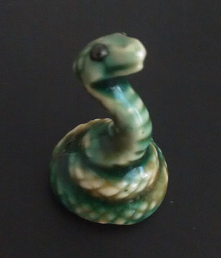
\includegraphics[scale=1]{ular-png}  
	\caption[Gambar {\it Serpentes} dalam format png]{Gambar {\it Serpentes} dalam format png} 
	\label{fig:ularpng} 
\end{figure} 

\dtext{19-20}
\begin{figure}[H]
	\centering  
	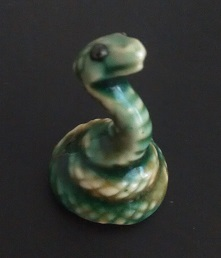
\includegraphics[scale=0.5]{ular-jpg}  
	\caption[Ular kecil]{Ular kecil} 
	\label{fig:ularjpg} 
\end{figure} 
\dtext{21-22}

\begin{figure}[ht] 
	\centering  
	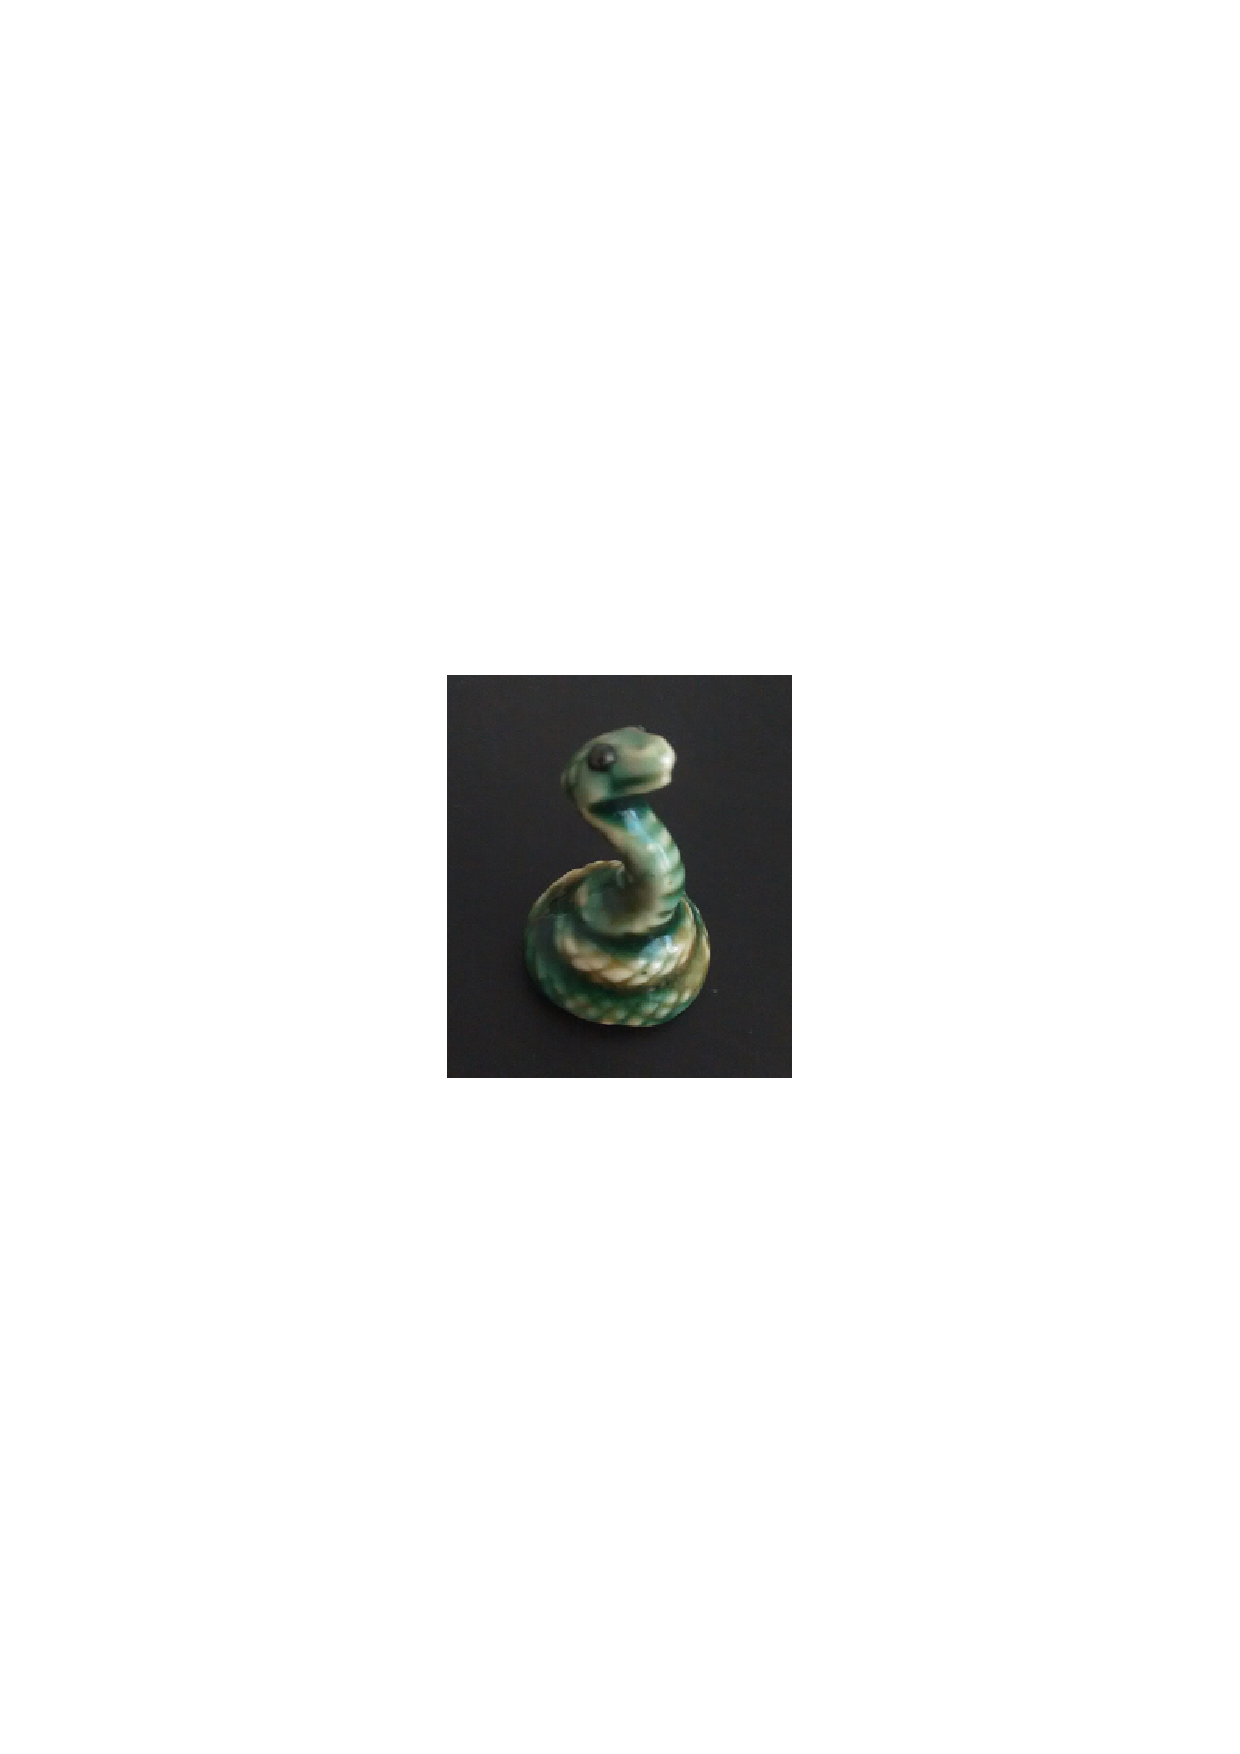
\includegraphics[scale=1]{ular-pdf}  
	\caption[ {\it Serpentes} betina]{ {\it Serpentes} jantan} 
	\label{fig:ularpdf} 
\end{figure} 
 
